\chapter{Self-hosted Oracle Implementation} \label{chap:concl}

\section*{}

In this chapter I present a possible implementation of a multi-purpose self-hosted oracle. Multi-purpose since it will be able to query a requested API and return a specific key from the answer of that API, allowing to be used by several contracts which require different information and different sources. Self-hosted, as its code is available for anyone to copy and use for their own purpose and not having to rely on and oracle-as-a-service product.

As far as the author as searched, at the moment there is no clear explanation on how to implement your own oracle and therefore on how to power smart-contracts to query the web. Creating, therefore, a need for such a clear and detailed explanation as it will be presented in this section.

In principle, the described oracle is intended to be used by single entities or competing parties. Meaning, that it requires a list of predefined oracles and a predefined minimum quorum. Therefore, is not open to a community in which oracles can leave and join the network. The rationale behind this decision is that if it were to be open to a community the decision power in the final result would be dependent on who could launch the most oracles, solving this issue would require  the use of strategies, such as, proof-of-work which would become a different issue that the one the author is trying to solve.
In this setup, competing parties which may not trust each other, would be able to power their contracts by having each party launching one oracle, and therefore having all the same power of decision. Has the list of the oracles address is in the open on the oracle smart contract, there is no way for a party to cheat in their voting power.

\section{Oracle Overview}

The oracle compromises two main components, the on-chain oracle and the off-chain oracle. Figure \ref{fig:/figures/self-hosted-architecture} depicts the general architecture and a simplified version of the messages exchanged.

\begin{figure*}[t]
    \begin{center}
        \leavevmode
        \includegraphics[width=1\textwidth]{figures/self-hosted-architecture.png}
        \caption{Self-hosted architecture.}
        \label{fig:/figures/self-hosted-architecture}
    \end{center}
\end{figure*}


The on-chain oracle is a smart contract which is the bridge between a client smart contract which needs to query the web and the oracle service which will query the web. This oracle has a whitelist of oracle addresses which are trusted by the oracle to query the web and has the necessary functions to create events that will trigger API calls and reach a consensus and the necessary data structures to store the requests and the agreed answer.

The off-chain oracle, or oracles, are services that continuously listen to specific events emitted by the oracle smart contract. Upon listening to a \textit{NewRequest} event query the specified API and key and return a single value to the smart contract by means of a new transaction.

This architecture allows for Nonetheless, the higher the number of oracles the higher the cost per request. Table 5.7 shows thecost each query using different numbers of oracles.several oracle nodes and different minimum vNonetheless, the higher the number of oracles the higher the cost per request. Table 5.7 shows thecost each query using different numbers of oracles.ms to achieve higher levels of trust, incluNonetheless, the higher the number of oracles the higher the cost per request. Table 5.7 shows thecost each query using different numbers of oracles.ties or increase service availability. NonetheNonetheless, the higher the number of oracles the higher the cost per request. Table 5.7 shows thecost each query using different numbers of oracles.igher the number of oracles the higher the cosNonetheless, the higher the number of oracles the higher the cost per request. Table 5.7 shows thecost each query using different numbers of oracles.st. Table \ref{oracle-query-cost} shows theNonetheless, the higher the number of oracles the higher the cost per request. Table 5.7 shows thecost each query using different numbers of oracles.ch query using different numbers of oracles.Nonetheless, the higher the number of oracles the higher the cost per request. Table 5.7 shows thecost each query using different numbers of oracles.

\begin{figure}[H]
    \centering
    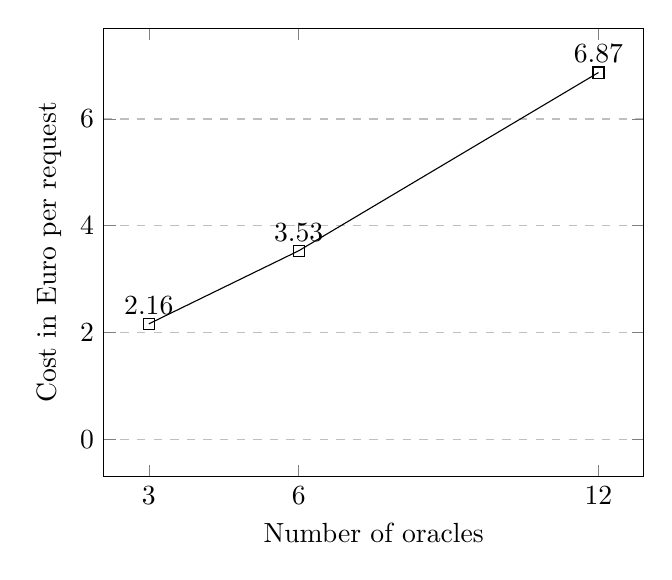
\begin{tikzpicture}
        \begin{axis}[
                xlabel={Number of oracles},
                ylabel={Cost in Euro per request},
                xtick=data,
                x tick label style={
                        /pgf/number format/1000 sep=},
                xmin=3, xmax=12,
                ymin=0, ymax=7,
                ytick={0,2,4,6,8},
                ymajorgrids=true,
                grid style=dashed,
                enlargelimits=0.10,
            ]

            \addplot[
                mark=square, nodes near coords
            ]
            coordinates {
                    (3,2.16)(6,3.53)(12,6.87)
                };

        \end{axis}
    \end{tikzpicture}
    \caption{Cost per query using a consensus of 2/3,}{Queried Google Finance on the 22th of May, 2019.}
    \
    \label{oracle-query-cost}
\end{figure}

\section{Component analysis}


\subsection{On-Chain Oracle}

The on-chain oracle is a smart contract that has an array which stores the requests made to the contract. Hard-coded in the contract is the predefined minimum quorum, which is the minimum number of equal answers needed to trust in the declaration of a final result. This minimum quorum will be used in all requests to the contract.
Also hard-coded are the white-listed addresses of oracles that the contract will accept transactions to update requests.

Initially the request structure \ref{code:request-struct} only contains the URL which will be queried by the off-chain oracle and the attribute to return in the json API response.

\begin{lstlisting}[language=Solidity, label=code:request-struct]
  struct Request {
    uint id;                            //request id
    string urlToQuery;                  //API url
    string attributeToFetch;            //json attribute (key) to retrieve in the response
    string agreedValue;                 //value from key
    mapping(uint => string) anwers;     //answers provided by the oracles
    mapping(address => uint) quorum;    //oracles which will query the answer (1=oracle hasn't voted, 2=oracle has voted)
  }
\end{lstlisting}


\section{Summary and Conclusions}